\chapter{RECOLECCIÓN DE LA INFORMACIÓN}

\section{Recolección y ordenamiento de información}

La búsqueda de la información se realiza con base en los elementos del problema, las variables intervinientes en el proceso y los indicadores. Se hace necesario que como investigadores y responsables de estas acciones se tenga un dominio conceptual y teórico tanto del tema objeto de investigación, como de la población a estudiar, para minimizar la posibilidad de que se presenten sesgos en esta etapa. 

\vspace{0.5cm}

La recolección de la información se realiza utilizando el proceso planeado paso a paso, para que de forma coherente se obtengan los resultados que contribuyen favorablemente al logro de los objetivos propuestos. 

\subsubsection{Información materia prima para la investigación}

Para el proceso de investigación se tomo la población de los conjuntos residenciales de la constructora AR del barrio perdomo. La información fue recopilada por medio de la técnica de cuestionarios que fueron elaborados con la herramienta de formlarios de Google. La muestra para la investigación es de 129 personas encuestadas.

\vspace{0.5cm}

Se pretende capturar la esencia del proceso por medio de la experiencia propia vivida al interior de las propiedades horizontales esto por medio de la observación. Las encuestas permiten capturar a mayor detalle lo vivido por cada uno de los participantes en el proceso, al igual que las entrevistas. Los cuestionarios permiten realizar preguntas puntuales y no se requiere que sea el investigador el que realice esta tarea, esto lo puede realizar cualquier persona involucrada o no en el proceso.


\section{Tabulación, ordenamiento y procesamiento de la información}

Para el análisis de la información recopilada se realiza la codificación de manera numérica a cada una de las alternativas de respuestas presentadas en el cuestionario realizado a los copropietarios de propiedad horizontal y de esta manera poder facilitar la tabulación de los resultados y el conteo de datos.

A continuación se presenta la información códificada:

\begin{longtable}{|l|l|l|l|} 
		\hline
		\multicolumn{4}{|l|}{\textbf{Codificación}}                                                                                                                                                                                                                                       \\ 
		\hline
		\textbf{\begin{tabular}[c]{p{1cm}@{}l@{}} Item   \end{tabular}}                               & \textbf{Pregunta}                                                                                                                                                                          & \textbf{\centering \begin{tabular}[c]{p{1cm}@{}l@{}} SUB ITEM   \end{tabular}} & \textbf{\centering Respuesta}  \\ 
		\hline
		\multirow{2}{*}{1}                          & \multirow{2}{*}{\begin{tabular}[c]{p{9cm}@{}l@{}}¿El registro para el ingreso a la asamblea es organizado y rápido? \end{tabular}} & 1.1              & SI                  \\ 
		\cline{3-4}
		&                                                                                                                                                                                            & 1.2              & NO                  \\ 
		\hline
		\multirow{2}{*}{2~}                         & \multirow{2}{*}{\begin{tabular}[c]{p{9cm}@{}l@{}}La forma más efectiva de votación es: \end{tabular}}                                                                                        & 2.1              & PAPEL               \\ 
		\cline{3-4}
		&                                                                                                                                                                                            & 2.2              & ELECTRÓNICO         \\ 
		\hline
		\multirow{2}{*}{3}                          & \multirow{2}{*}{\begin{tabular}[c]{p{9cm}@{}l@{}}¿La presentación de los resultados de la Asamblea General es ágil y eficiente? \end{tabular}}                                                 & 3.1              & SI                  \\ 
		\cline{3-4}
		&                                                                                                                                                                                            & 3.2              & NO                  \\ 
		\hline
		\multirow{2}{*}{4}                          & \multirow{2}{*}{\begin{tabular}[c]{p{9cm}@{}l@{}}¿Actualmente cuenta con un celular Smartphone? \end{tabular}}                                                                                 & 4.1              & SI                  \\ 
		\cline{3-4}
		&                                                                                                                                                                                            & 4.2              & NO                  \\ 
		\hline
		\multirow{2}{*}{5}                          & \multirow{2}{*}{\begin{tabular}[c]{p{9cm}@{}l@{}}¿La duración de las Asambleas Generales es el adecuado? \end{tabular}}                                                                        & 5.1              & SI                  \\ 
		\cline{3-4}
		&                                                                                                                                                                                            & 5.2              & NO                  \\ 
		\hline
		\multirow{2}{*}{6}                          & \multirow{2}{*}{\begin{tabular}[c]{p{9cm}@{}l@{}}¿Cree que el conteo de los votos actualmente es confiable? \end{tabular}}                                                                     & 6.1              & SI                  \\ 
		\cline{3-4}
		&                                                                                                                                                                                            & 6.2              & NO                  \\ 
		\hline
		\multirow{2}{*}{7}                          & \multirow{2}{*}{\begin{tabular}[c]{p{9cm}@{}l@{}}¿Cree que una aplicación o sistema podría mejorar la efectividad de la asamblea? \end{tabular}}                                               & 7.1              & SI                  \\ 
		\cline{3-4}
		&                                                                                                                                                                                            & 7.2              & NO                  \\
		\hline
		\caption{Tabulación de la información}
\end{longtable}


Para la Tabulación de los datos recopilados consiste en el recuento de las respuestas contenidas en la encuesta, a través del conteo de los códigos númericos de las alternativas de respuestas codificadas, con la finalidad de generar los resultados que se presentan a continuación:

\vspace{1cm}

\begin{longtable}[h!]{|l|l|l|l|} 
	\hline
	\multicolumn{4}{|c|}{\textbf{Tabulación}}                                                                                                                                                                                                                                       \\ 
	\hline
	\textbf{\begin{tabular}[c]{p{1cm}@{}l@{}} ITEM   \end{tabular}}                               & 
	\textbf{\begin{tabular}[c]{p{1cm}@{}l@{}} SUB ITEM   \end{tabular}} & \textbf{Respuesta} & \textbf{Total}  \\ 
	\hline
	\multirow{2}{*}{1} & 1.1 & SI & 8 \\ 
	\cline{3-4}  & 1.2 & NO & 121   \\ 
	\hline
	\multirow{2}{*}{2~} & 2.1  & PAPEL & 11 \\ 
	\cline{3-4} & 2.2  & ELECTRÓNICO & 118  \\ 
	\hline
	\multirow{2}{*}{3} & 3.1   & SI  & 8 \\ 
	\cline{3-4} &  3.2  & NO  & 121  \\ 
	\hline
	\multirow{2}{*}{4} & 4.1  & SI  & 118 \\ 
	\cline{3-4} & 4.2 & NO & 11 \\ 
	\hline
	\multirow{2}{*}{5} &  5.1 & SI & 6 \\ 
	\cline{3-4} & 5.2 & NO & 123 \\ 
	\hline
	\multirow{2}{*}{6}  & 6.1 & SI & 15 \\ 
	\cline{3-4}  & 6.2 & NO & 114 \\ 
	\hline
	\multirow{2}{*}{7} & 7.1 & SI & 120\\ 
	\cline{3-4} & 7.2 & NO & 9 \\
	\hline	
	\caption{Ordenamiento de la información}
\end{longtable}



\subsubsection{Ordenamiento}

El ordenamiento para el tipo de encuesta realizada se genera por ponderación asignada a cada pregunta, con esto se representa el nivel de importancia que tiene la pregunta para la investigación. Las ponderaciones se generan desde el número uno hasta el número 7, siendo la ponderación 1 como la más importante y relevante, y la ponderación 7 la de menor valor.

\vspace{0.5cm}

\begin{longtable}[c]{|p{7.5cm}|c|}
	\hline
	\multicolumn{2}{|c|}{\textbf{Ordenamiento}}                                                          \\ \hline
	\multicolumn{1}{|c|}{\textbf{Pregunta}}                                          & \textbf{Ponderado} \\ \hline
	¿El registro para el ingreso a la asamblea es organizado y rápido?               & \textbf{1}        \\ \hline
	La forma más efectiva de votación es:                                            & \textbf{2}        \\ \hline
	¿Cree que una aplicación o sistema podría mejorar la efectividad de la asamblea? & \textbf{5}        \\ \hline
	¿Actualmente cuenta con un celular Smartphone?                                   & \textbf{7}        \\ \hline
	¿La duración de las Asambleas Generales es el adecuado?                          & \textbf{4}        \\ \hline
	¿Cree que el conteo de los votos actualmente es confiable?                       & \textbf{3}        \\ \hline
	¿Cree que una aplicación o sistema podría mejorar la efectividad de la asamblea? & \textbf{6}        \\ \hline
	\caption{Ordenamiento}
\end{longtable}

\section{Presentación de resultados}

\subsubsection{Resultados}

Los resultados de cada preguntas se presentarán gárico de Torta, facilitando su lectura, al contar solo con dos opciones de respuesta la represetnación gráfica es sencilla y permite su mayor comprensión.

\vspace{0.5cm}

Cada una de las preguntas era comprensible para la persona encuesta y brindo resultados que permitieron comprobar que el foco de la investigación se había seleccionado de manera adecuada.

\vspace{0.5cm}

Las preguntas realizadas con el total de votos fueron las siguientes:

\begin{itemize}
	\item ¿Cree que una aplicacion o sistema podria mejorar la efectividad de la asamblea? (SI=8 - NO=121).
	
	\item La forma más efectiva de votación es: (PAPEL=11 - ELECTRÓNICO=118)
	
	\item La presentación de los resultados de la Asamblea General es ágil y eficiente? (SI=8 - NO=121).
	
	\item Actualmente cuenta con un celular Smartphone?(SI=118 - NO=11).
	
	\item ¿La duración de las Asambleas Generales es el adecuado? (SI=6 - NO=123).
	
	\item ¿Cree que el conteo de los votos actualmente es confiable? (SI=15 - NO=114).
	
	\item ¿Cree que una aplicacion o sistema podria mejorar la efectividad de la asamblea? (SI=120 - NO=9).
\end{itemize}


\subsubsection{Gráficos}

A continuación se presenta un ejemplo de las gráficas elaboradas para la presentación de resultados:

%%grafo

\begin{figure}[th!]
	\centering
	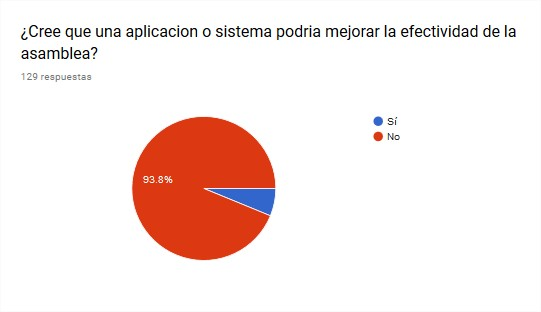
\includegraphics[width=7cm,height=3.5cm]{desarrollo/resultados/imgs/pregunta-1}
	\caption{Gráfica pregunta 1}{\scriptsize \textbf{Fuente:} Imagen propia}
\end{figure}